% !TEX root = ../main.tex
%
\chapter{Methodology}
\label{sec:methodology}

This research was organized into three sequential phases: initial user research, prototype development, and user testing. 
Each phase was designed to inform and refine the subsequent stages, ensuring a systematic approach to developing a user-friendly NeRF interface. 
This iterative process aimed to align closely with user needs and feedback, fostering a design that is both intuitive and functional.

\section{Initial User Research}
\label{sec:methodology:user-research}

The foundational stage of this research involved conducting a series of in-depth interviews to gather insights into the user experience of NeRF technology. 
The primary objective was to understand the varied challenges, needs, and preferences of users, ranging from novices to experts in NeRF model creation, particularly those with ties to the film industry. 
This exploratory phase was crucial for identifying the key features and improvements necessary for a more accessible and efficient NeRF interface.

\subsection*{Participant Selection Criteria}
\label{sec:methodology:user-research:criteria}

Participants were carefully chosen based on their prior experience with NeRF technology and their connection to the film industry, culminating in a group of four experts. 
This selection ensured a rich diversity of perspectives, encompassing a broad spectrum of technical proficiency and practical applications of NeRF. 
By including individuals who have utilized NeRF in various capacities, the study aimed to uncover both the shared challenges faced by all users and the unique requirements of distinct user groups within the film industry.

\subsection*{Interview Methodology}
\label{sec:methodology:user-research:interview}

The interviews were designed as semi-structured conversations, following a core set of predetermined questions (see Appendix \ref{sec:appendix:interview-questions}) while also allowing for spontaneous discussions and additional queries. 
Conducted one-on-one, these interviews facilitated a personalized dialogue with each participant, offering insights into individual experiences and perspectives. 
Although the interviews were prepared in English, all conversation were held in German, to ensure comfort and clarity for participants, potentially leading to more candid and informative discussions.

The structured flow of questions began with learning about the participants' backgrounds and experiences with NeRF technology, gradually moving towards more detailed questions about their specific needs, challenges, and desired improvements in NeRF interfaces. 
Participants were also invited to propose features or functionalities they believed would enhance the usability and effectiveness of a NeRF interface for their professional or academic projects.

To ensure a comprehensive analysis, interviews were recorded and transcribed with participants' consent, allowing for a detailed review and coding of the responses. 
This process enabled the identification of recurring themes, challenges, and preferences across the participant group, providing a solid foundation for the subsequent phases of prototype development and user testing. 
The insights gained from this initial research phase were instrumental in shaping the direction and focus of the interface design, ensuring it would effectively address the real-world needs of NeRF users.

\subsection*{Key Findings}
\label{sec:methodology:user-research:findings}

\paragraph{NeRF in the Film Industry}

NeRF technology is being explored for various applications in the film industry, such as visual effects, virtual production, and pre-production location scouting. 
Despite its potential to simplify the creation of 3D scenes, current limitations in model quality, lack of editable models, and insufficient detail hinder its professional use. 
However, its capability for quick 3D scene captures offers significant benefits for pre-visualization and planning in the pre-production phase, although concerns about model scale accuracy for export remain.

\paragraph{Optimizing Parameters and Workflow}

Creating NeRFs typically involves preprocessing input data, training models, and exporting outputs. 
Technical users emphasize the importance of parameter optimization in improving NeRF quality, with iterative training and results analysis being crucial parts of their workflow. 
Tools like TensorBoard are utilized for quantifying variations in training outcomes.

\paragraph{User Interface and Accessibility}

A consensus among users highlights the need for an intuitive, all-encompassing user interface that minimizes reliance on console commands. 
Features that allow users to visually navigate and control the NeRF creation pipeline, including real-time progress feedback and the ability to pause and adjust processes at any stage, are highly valued.

\paragraph{Web-Based Interfaces and Collaboration}

Preferences have shifted towards web-based interfaces, facilitating remote project management and data handling. 
Such interfaces support collaborative efforts, allowing users to easily share and review project stages.

\paragraph{Comprehensive Error Handling and Visualization}

Effective error feedback and clear, informative visualization tools are critical for user satisfaction. 
Users express frustration with vague error messages and cumbersome command-line interactions for troubleshooting and adjustments.

\paragraph{File Management and Project Structure}

Efficient file and project management, with clear distinctions between different stages (preprocessing, training, rendering) and support for various input formats, is essential. 
Users discuss challenges with current tools regarding data organization, suggesting improvements for handling input data and managing projects​​.

% \paragraph{Quality, Performance, and Scalability}

% Concerns about the scalability of projects, particularly when dealing with large datasets or aiming for high-quality outputs, are prevalent. 
% Users desire improvements in performance management and quality assurance mechanisms.

\paragraph{Integration and Export Options}

Strong integration capabilities with popular 3D and VFX software and flexible export options are desired. 
Users discuss the importance of being able to easily import NeRF-generated scenes into tools like Unreal Engine or Blender for further processing and use in production-quality projects​​.

\paragraph{Multi-Mode Operation}

The necessity for multi-mode operation in NeRF tool interfaces emerges as a significant insight, underlining the importance of accommodating a broad spectrum of users, from novices to experts. 
A simplified mode is envisioned to cater to beginners, offering an intuitive and streamlined workflow, whereas an advanced mode is tailored for experienced users requiring detailed control over the NeRF creation process. 
% By embracing a multi-mode approach, NeRF tools can democratize access to sophisticated 3D modeling capabilities, fostering a creative and inclusive environment for users of all backgrounds.

\paragraph{Conclusion}

These findings highlight the demand for a NeRF tool interface that is user-friendly, versatile, and capable of supporting a wide range of workflows and user expertise levels. 
The ideal tool would combine intuitive project management and visualization features with powerful customization options, robust error handling and feedback mechanisms, and effective performance management capabilities.

\section{Design and Development Process}
\label{sec:methodology:design-development}

The transition from initial user research findings to a functional prototype was a multi-step process focused on capturing user needs and translating them into a tangible design. 
This section outlines the journey from abstract requirements to the creation of the prototype, emphasizing the methodologies employed at each step.

\subsection*{From User Research to User Flow Diagram}

Following the completion of initial user research, the first step involved modeling the key findings into a user flow diagram (Figure \ref{fig:design:flow-1}).
This diagram served as a visual representation of the user's journey through the prototype, highlighting the main actions, decisions, and interactions users would have with the system. 

\begin{figure}[htb]
	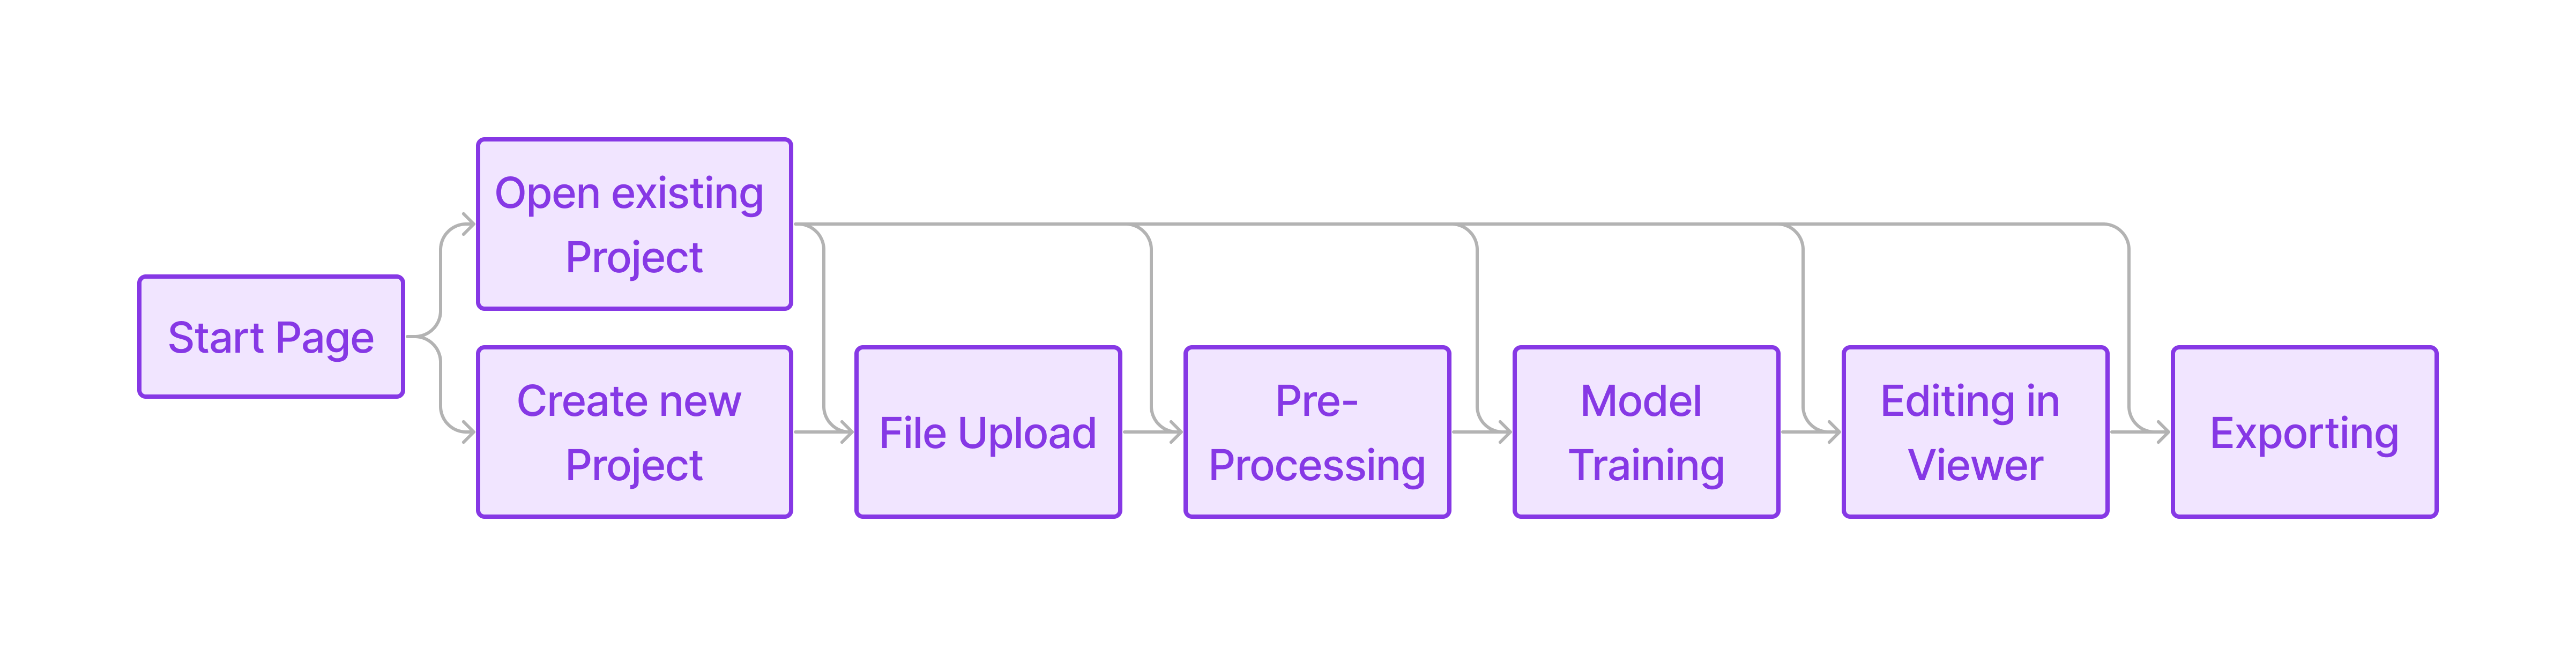
\includegraphics[width=\textwidth]{figures/flow-1.png}
	\caption{User Flow Diagram}
	\label{fig:design:flow-1}
\end{figure}

The purpose of the user flow diagram was not only to map out the envisioned user experience but also to identify any potential bottlenecks or usability issues early in the design process.

\subsection*{Developing the Site Map}

Building on the foundation laid by the user flow diagram, the next step was to expand this outline into a detailed site map. 
The site map provided a more comprehensive view of the prototype's structure, detailing the relationships between different pages and features. 
This excerpt from the site map (Figure \ref{fig:design:flow-2}) illustrates the level of detail and complexity involved in mapping out the prototype's user interactions.

\begin{figure}[htb]
  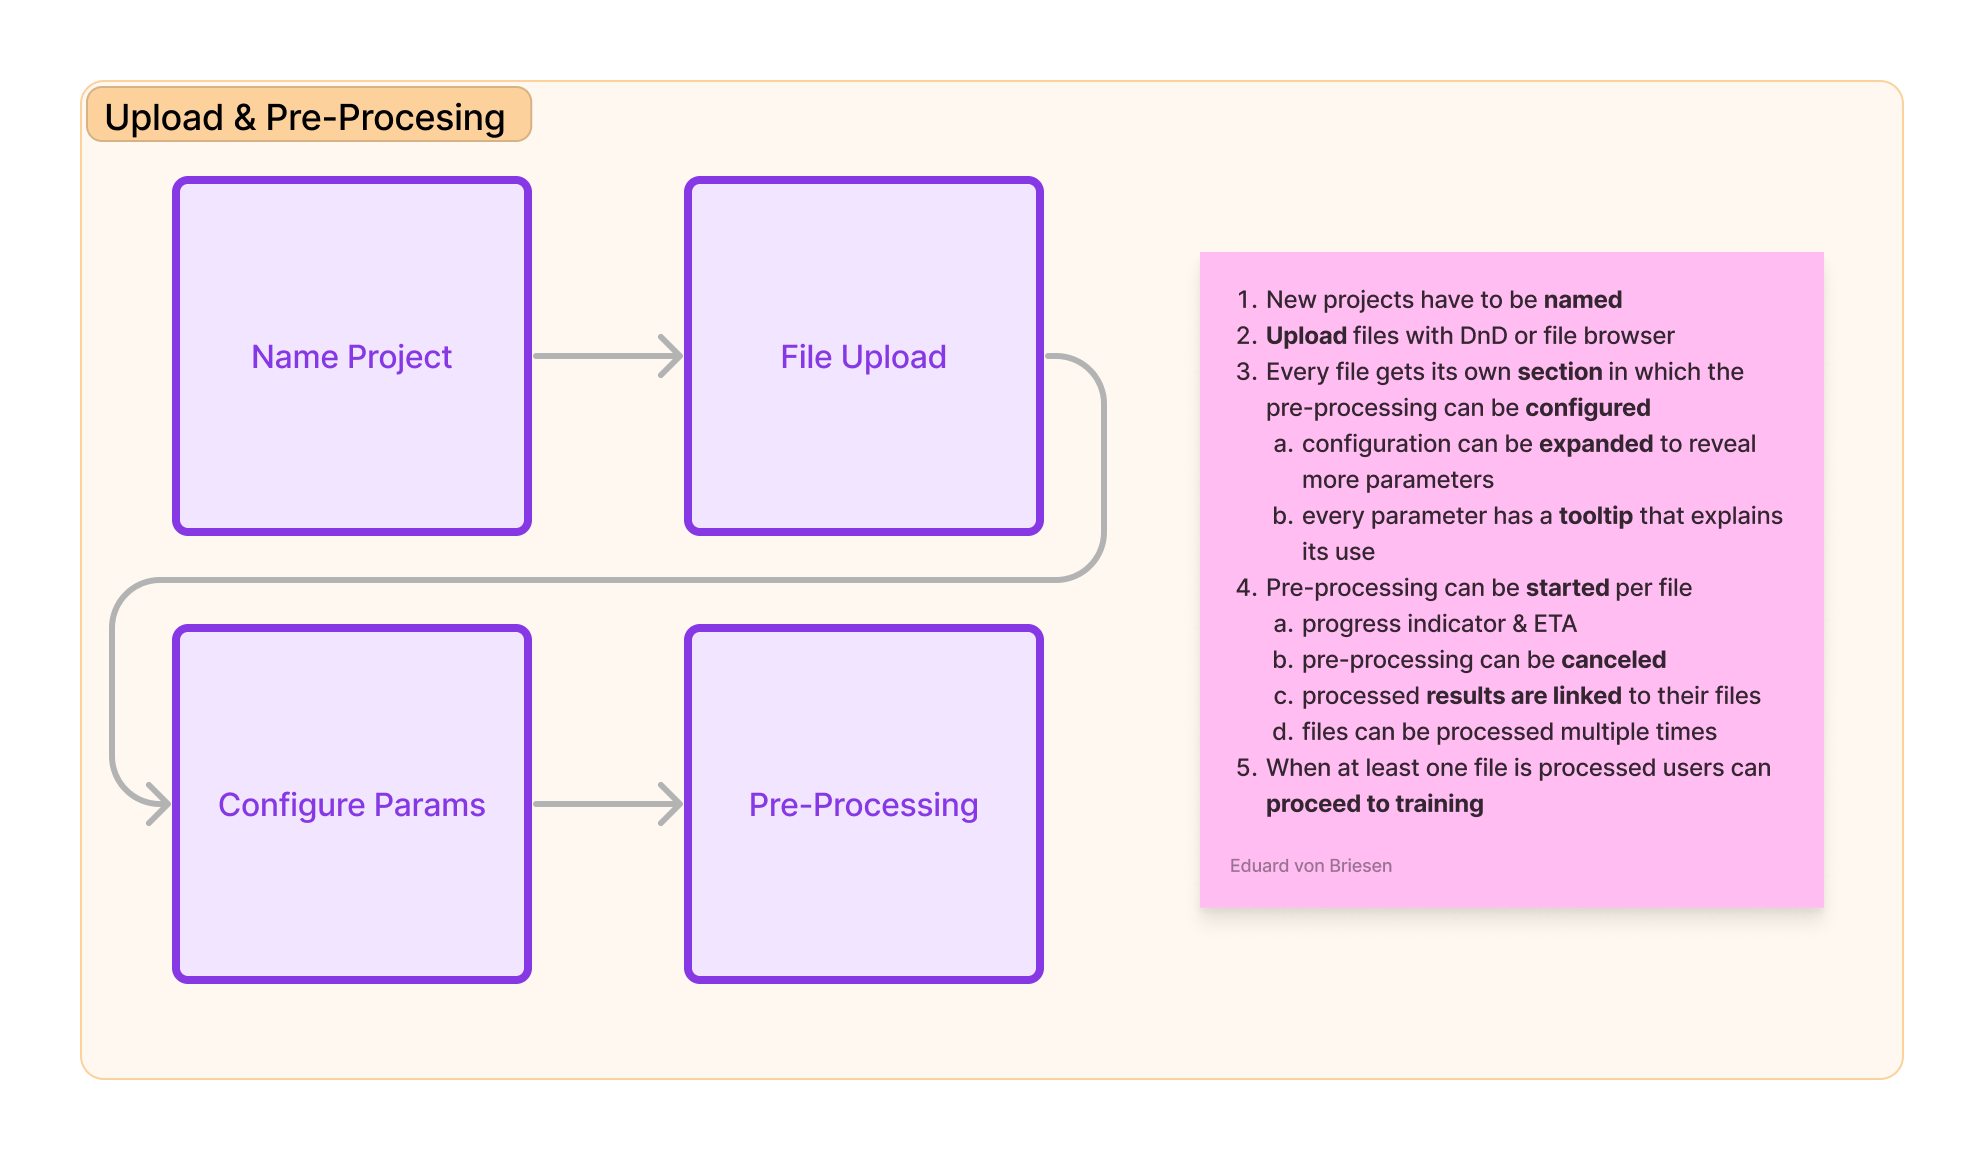
\includegraphics[width=\textwidth]{figures/flow-2.png}
  \caption{Excerpt of a View from the Flow Diagram with detailed interactions}
  \label{fig:design:flow-2}
\end{figure}

This expanded view was instrumental in ensuring that the user flow remained intuitive across the broader system, facilitating easy navigation and a cohesive user experience.

\subsection*{Wireframing}

With a solid understanding of the user flow and site structure, the focus shifted to wireframing. 
Initial wireframes were created to model the overall layout of the interface, providing a skeletal framework for the visual design. 
These wireframes were kept intentionally simple to prioritize structural and functional decisions over aesthetic considerations.
At this stage, emphasis was placed on the placement of key elements, usability, and adherence to the user flow and site map.

\begin{figure}[htb]
  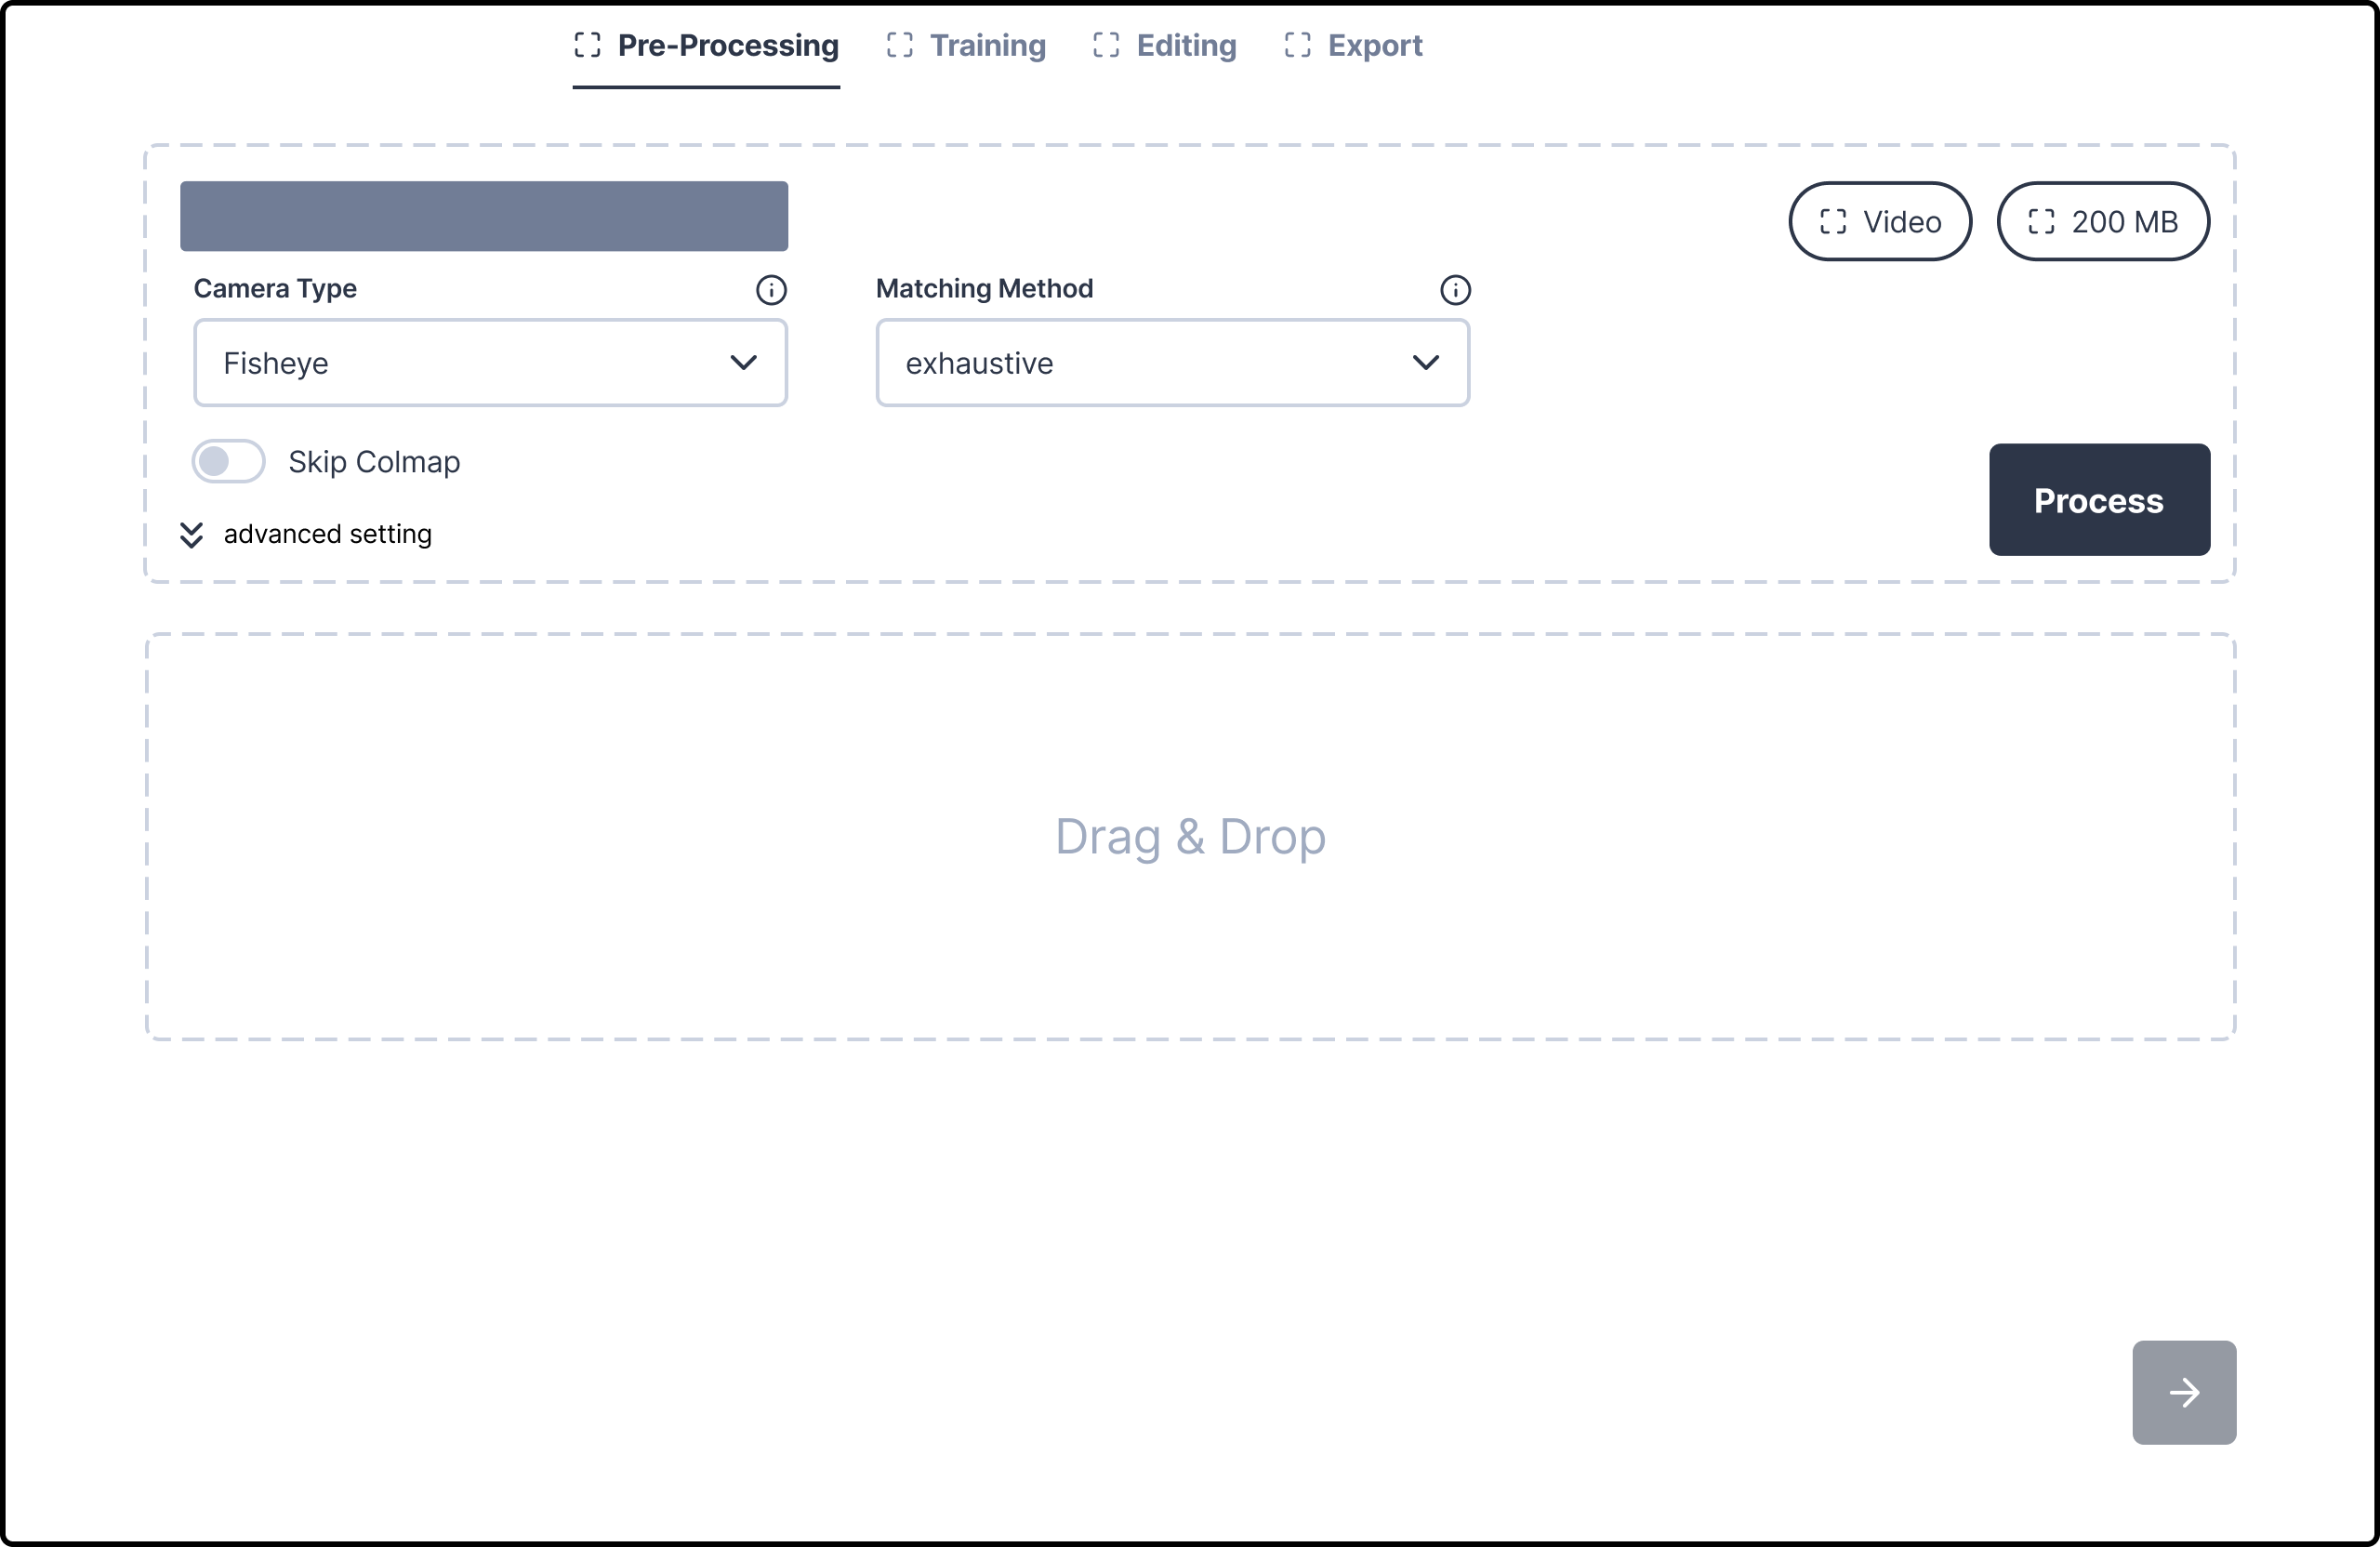
\includegraphics[width=\textwidth]{figures/wireframe.png}
  \caption{Wireframe of the Pre-Processing Section}
  \label{fig:design:wireframe}
\end{figure}

\subsection*{Refinement Through Development}

The transition from wireframes to a working prototype involved iterative refinement during the development phase. 
As the prototype took shape, initial designs were continuously evaluated and adjusted based on practical considerations and technical constraints. 
This phase allowed for a deeper exploration of interactions, animations, and the overall look and feel of the interface. 
It was during this time that the wireframes evolved into a more detailed and user-friendly interface, with adjustments made as necessary to enhance usability and ensure a seamless user experience.

\section{User Study and Evaluation}
\label{sec:methodology:study}

To evaluate the usability and overall utility of the developed NeRF interface prototype, a comprehensive user study was conducted. 
The primary aim of this study was to collect feedback on the prototype's user experience, identify any usability challenges participants encountered, and understand their satisfaction levels with the interface. 
Employing a mixed-methods approach allowed for a blend of quantitative and qualitative data collection and analysis, offering a multifaceted view of the prototype's performance in real-world tasks.
Participants were given a set of tasks to complete within the prototype, followed by a User Experience Questionnaire (UEQ) and a follow-up interview to gather detailed feedback on their experiences.

\subsection*{Tasks Based Usability Test}
\label{sec:methodology:study:tasks}

The usability test was conducted in a controlled environment, with participants being asked to complete a two tasks with the prototype.
The tasks were designed to cover a range of functionalities and features of the prototype, and represent a typical workflow when creating NeRF models.

\begin{enumerate}
  \item Task: Create a new project.
  \item Task: Upload a prepared video file.
  \item Task: Pre-process the uploaded file to prepare it for training.
  \item Task: Switch to an existing project that already pre-processed data.
  \item Task: Start a NeRF training.
  \item Task: Create a camera path in the viewer.
  \item Task: Export a video.
\end{enumerate}

To keep an appropriate time frame, none of the tasks required completion of a training process, and pre-processed data and pre-trained models were provided to the participants.
On average, participants took 30 minutes to complete the tasks.

Participant were passively observed while working on their tasks, to identify any problems or operation errors they encountered and to determine their overall performance.
In addition the screen was recorded to capture the participants interactions with the prototype, and to allow for a more detailed analysis of their behavior later on.

\subsection*{User Experience Questionnaire}
\label{sec:methodology:study:ueq}

After completing their tasks, users were asked to fill out the User Experience Questionnaire (UEQ) \cite{laugwitz_construction_2008}, a standardized questionnaire for the assessment of user experience.
It measure user experience in six dimensions:

\begin{itemize}
  \item \textbf{Attractiveness} - the overall impression of the product
  \item \textbf{Perspicuity} - the clarity and understandability of the product
  \item \textbf{Efficiency} - the perceived effort required to use the product
  \item \textbf{Dependability} - the perceived reliability and trustworthiness of the product
  \item \textbf{Novelty} - the perceived originality and innovation of the product
  \item \textbf{Stimulation} - the perceived level of excitement and engagement with the product
\end{itemize}

This covers both classical usability goals (Efficiency, Perspicuity, Dependability) and user experience qualities (Novelty, Stimulation).
Attractiveness is purely a valence dimension, and is not directly related to usability or user experience.

In total the questionnaire consists of 26 items, each represented by two terms of opposite meaning. 
The order of the terms is randomized for each item, to avoid bias.
Participants are asked to rate each item on a 7-point scale, from -3 to +3, with 0 representing a neutral response.
An example of the scale can be seen below:

\begin{center}
  boring \quad o o o o o o o \quad exciting
\end{center}

The format of the questionnaire gives participants a clear and simple way to  quickly express their feelings and thoughts about the prototype, without much effort.

In this study the questionnaire was filled out by participants in digital form, using a web-based survey tool. %TODO: source
The survey included additional questions to gather demographic information and to capture prior experience with NeRF and other 3D modeling tools.
This allowed for a more efficient data collection and analysis, across in-person and remote participants.

\subsection*{Follow-up Interview}
\label{sec:methodology:study:interview}

After completing the usability test, participants were engaged in a short follow-up interview, to gather more detailed feedback on their experience with the prototype. 
Similar to the initial user interviews, these interviews were semi-structured, following a pre-defined set of question, with room for participants to share their own thoughts and suggestions.
The questions can be categorized into general usability, tasks specific feedback and suggestions for improvement.
The interview template can be found in the appendix \ref{sec:appendix:questionnaire}.


\subsection*{Data Analysis}
\label{sec:methodology:study:analysis}

Both the recordings of the usability test and the follow-up interviews were analyzed to identify common themes and patterns in the feedback of participants.
The video recordings were coded to highlight any usability issues or challenges that participants encountered during the tasks.
The audio recordings of the interviews were transcribed and coded.
The data was then categorized and analyzed to identify common themes and patterns across the participants.

Analysis of the UEQ data was done using the standard procedure for the questionnaire.
The UEQ provides a data analysis tool in form of spreadsheet, that calculates all necessary values and visualizes the results.

In summary, this user study and evaluation was pivotal in validating the effectiveness of the NeRF interface prototype, uncovering valuable insights into its usability, and identifying opportunities for further refinement. 
The mixed-methods approach ensured a balanced assessment, capturing both the tangible aspects of interface interaction and the subjective experiences of the users, providing a solid foundation for the next stages of development.